\documentclass[a4paper, 14pt]{extarticle}
\usepackage[russian]{babel}
\usepackage[T1]{fontenc}
\usepackage{fontspec}
\usepackage{indentfirst}
\usepackage{enumitem}
\usepackage{graphicx}
\usepackage[
  left=20mm,
  right=10mm,
  top=20mm,
  bottom=20mm
]{geometry}
\usepackage{parskip}
\usepackage{titlesec}
\usepackage{xurl}
\usepackage{hyperref}
\usepackage{float}
\usepackage[
  figurename=Рисунок,
  labelsep=endash,
]{caption}
\usepackage[outputdir=build, newfloat]{minted}

\hypersetup{
  colorlinks=true,
  linkcolor=black,
  filecolor=blue,
  urlcolor=blue,
}

\renewcommand*{\labelitemi}{---}
\setmainfont{Times New Roman}
\setmonofont{JetBrains Mono}[
  SizeFeatures={Size=11},
]

\newenvironment{code}{\captionsetup{type=listing}}{}
\SetupFloatingEnvironment{listing}{name=Листинг}

\setminted{
  fontsize=\footnotesize,
  frame=lines,
  framesep=2mm,
}

\setlength{\parskip}{6pt}

\setlength{\parindent}{1cm}
\setlist[itemize]{itemsep=0em,topsep=0em,parsep=0em,partopsep=0em,leftmargin=2.0cm,wide}
\setlist[enumerate]{itemsep=0em,topsep=0em,parsep=0em,partopsep=0em,leftmargin=2.0cm,wide}

\renewcommand{\thesection}{\arabic{section}.}
\renewcommand{\thesubsection}{\thesection\arabic{subsection}.}
\renewcommand{\thesubsubsection}{\thesubsection\arabic{subsubsection}.}

\titleformat{\section}{\normalfont\bfseries}{\thesection}{0.5em}{}
\titleformat{\subsection}{\normalfont\bfseries}{\thesubsection}{0.5em}{}

\titleformat*{\section}{\normalfont\bfseries}
\titleformat*{\subsection}{\normalfont\bfseries}

\linespread{1.5}
\renewcommand{\baselinestretch}{1.5}

\begin{document}

\begin{titlepage}
  \vspace{0pt plus2fill}
  \noindent

  \vspace{0pt plus6fill}
  \begin{center}
    Санкт-Петербургский национальный исследовательский университет
    информационных технологий, механики и оптики

    \vspace{0pt plus3fill}

    Факультет инфокоммуникационных технологий

    Направление подготовки 11.03.02

    \vspace{0pt plus2fill}

    Лабораторная работа №4

    <<Разработка веб-страницы>>

  \end{center}

  \vspace{0pt plus9fill}
  \begin{flushright}
    Выполнил: \\
    Швалов Даниил Андреевич

    Группа: К33211

    Проверила: \\
    Марченко Елена Вадимовна
  \end{flushright}

  \vspace{0pt plus2fill}
  \begin{center}
    Санкт-Петербург

    2023
  \end{center}
\end{titlepage}

\section{Введение}

\textbf{Цель работы}: научиться создавать веб-страницы с помощью HTML, CSS и
PHP-скриптов, которые взаимодействуют с базой данных MySQL.

\section{Ход работы}

В данной лабораторной работе необходимо написать две веб-страницы: страницу
оформления заказа, а также страницу входа в аккаунт. С точки зрения архитектуры
сайта это две разные страницы, которые не могут являться точкой входа для
пользователя. Поэтому в качестве главной страницы была создана страница, которая
встречает пользователя двумя кнопками: <<Вход в аккаунт>> и <<Оформление
заказа>> (см. рис \ref{fig:index.html}). Исходный код главной страницы находится
в приложении \ref{app:index.html}.

\begin{figure}[H]
  \centering
  \fbox{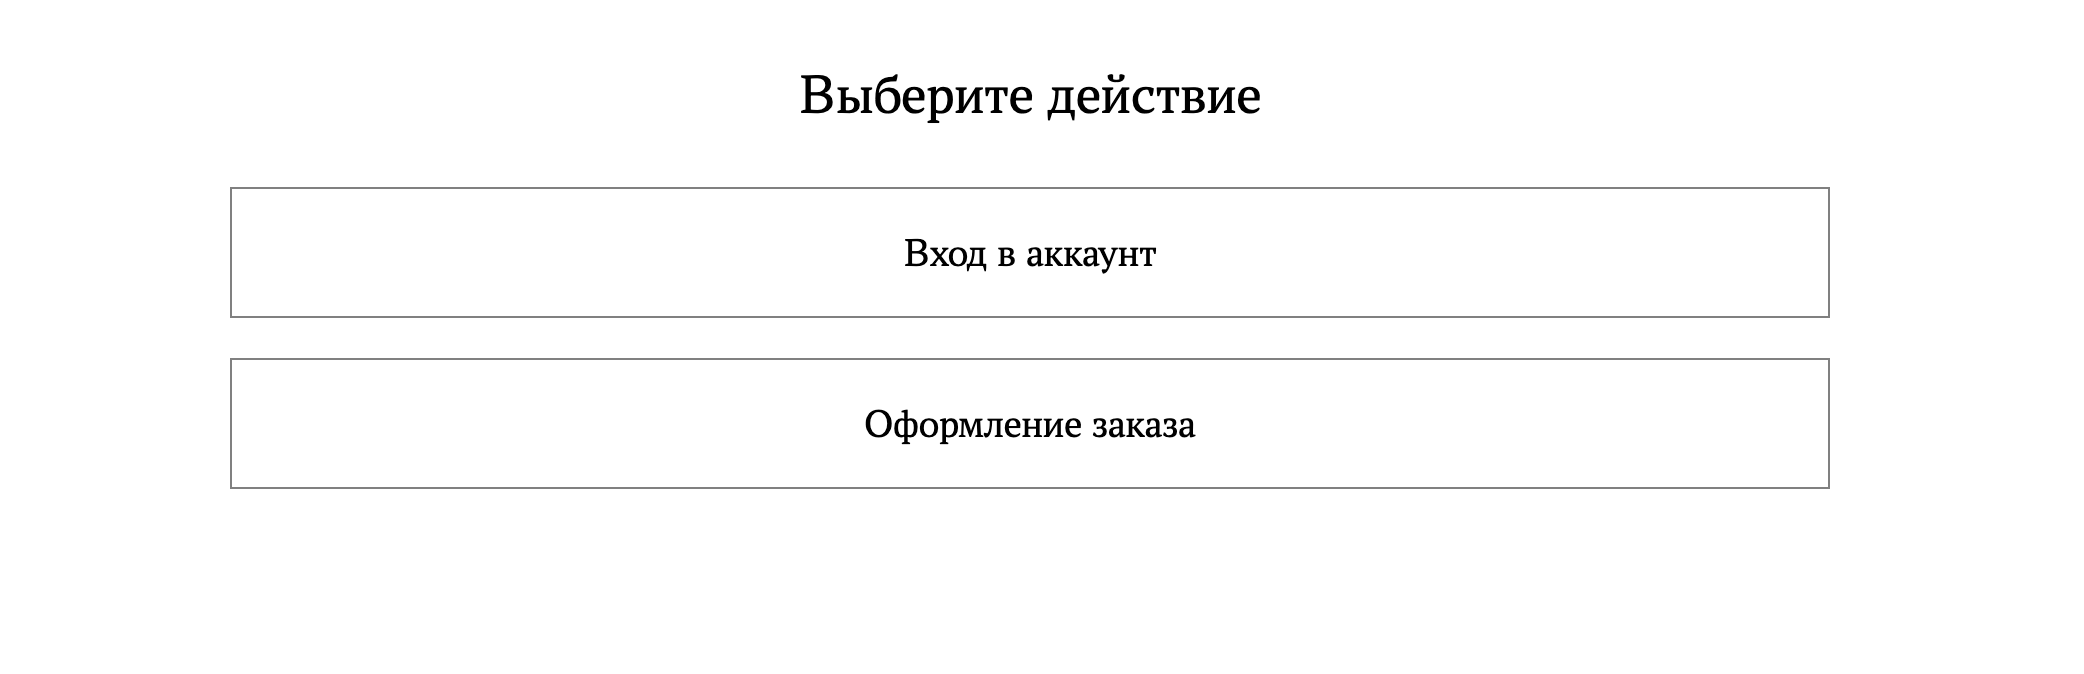
\includegraphics[width=0.9\textwidth]{images/index.png}}
  \caption{Главная страница}
  \label{fig:index.html}
\end{figure}

При нажатии на кнопку <<Вход в аккаунт>> пользователь попадает на страницу входа
в аккаунт (см. рис. \ref{fig:login.html}). На ней пользователю предлагается
ввести электронную почту и пароль, чтобы авторизоваться в аккаунт. После ввода
данных и нажатия кнопки <<Войти>>, запускается PHP-скрипт, обрабатывающих вход в
аккаунт. Исходный код страницы входа в аккаунт находится в приложении
\ref{app:login.html}.

\begin{figure}[H]
  \centering
  \fbox{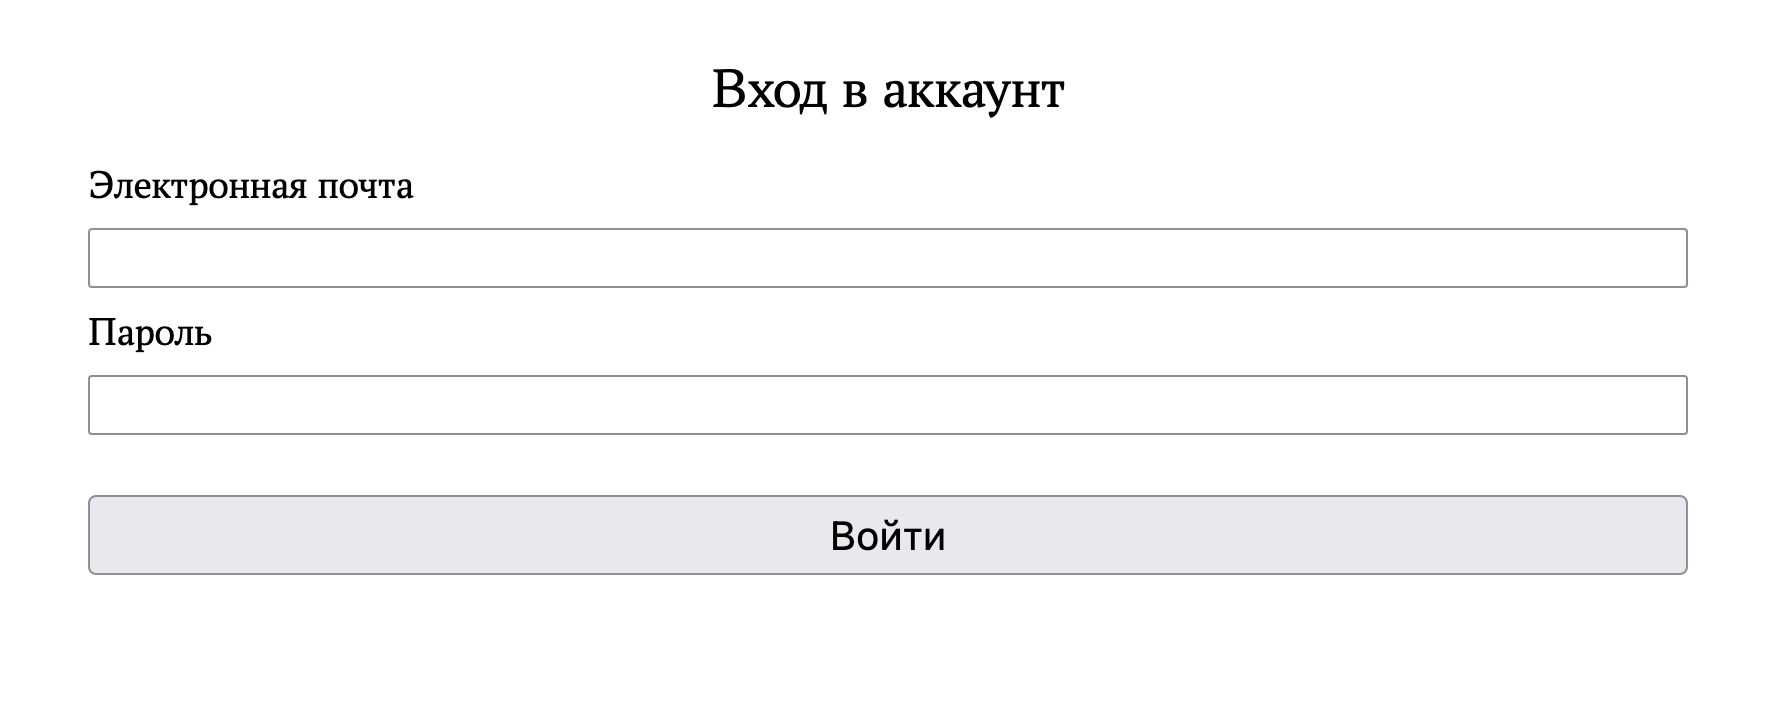
\includegraphics[width=0.9\textwidth]{images/login.png}}
  \caption{Страница входа в аккаунт}
  \label{fig:login.html}
\end{figure}

По условию задания первый вход в аккаунт должен создавать новую запись в базе
данных, поэтому вход в аккаунт работает как регистрация. Если пользователь с
таким почтовым адресом уже есть в базе данных, то новая запись не создается, а
сохраняется старая. Исходный код PHP-скрипта находится в приложении
\ref{app:login.php}.

После того, как PHP-скрипт отработал, пользователя перекидывает на страницу,
уведомляющую о том, что вход успешно совершен (см. рис.
\ref{fig:login-success.html}). После этого пользователь, нажав на кнопку
<<Вернуться на главную>>, может перейти обратно на главную страницу. Исходный
код страницы успешного входа в аккаунт находится в приложении
\ref{app:login-success.html}.

\begin{figure}[H]
  \centering
  \fbox{
\includegraphics[width=0.6\textwidth]{images/login-success.png}}
  \caption{Страница успешного входа в аккаунт}
  \label{fig:login-success.html}
\end{figure}

Если пользователь на главной странице (см. рис. \ref{fig:index.html}) нажал
кнопку <<Оформление заказа>>, то его перекидывает на страницу оформления заказа
(см. рис. \ref{fig:order.html}). На ней пользователю предлагается выбрать один
из товаров, который он хочет приобрести, а также ввести свою фамилию, имя,
отчество, адрес электронной почты, телефонный номер, а также физический адрес.
Также пользователь может оставить комментарий к заказу при необходимости. При
нажатии кнопки <<Отправить>> запускается PHP-скрипт, который обрабатывает
создание заказа.

\begin{figure}[H]
  \centering
  \fbox{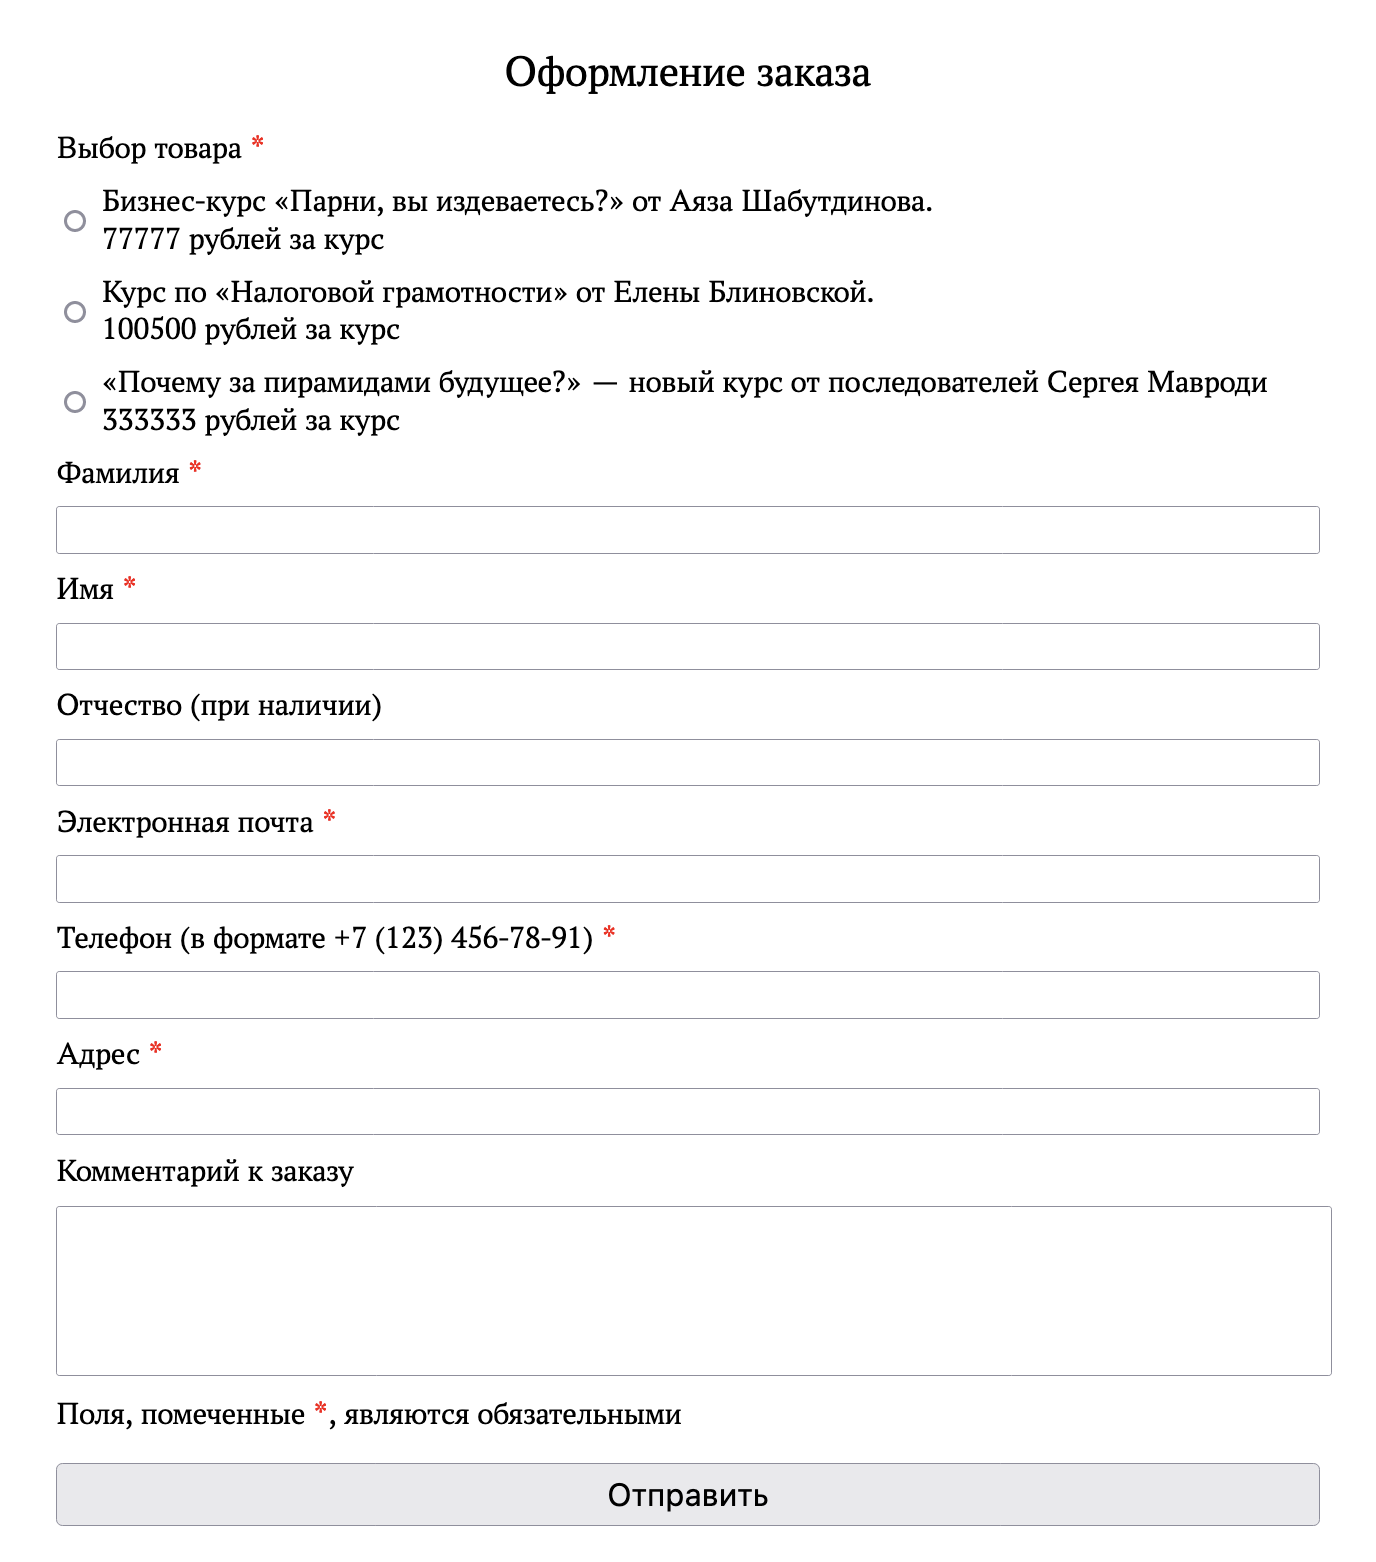
\includegraphics[width=0.9\textwidth]{images/order.png}}
  \caption{Страница оформления заказа}
  \label{fig:order.html}
\end{figure}

Так как веб-страница обладает достаточно скромным функционалом, проверка на то,
что оформление заказа производит авторизованный пользователь, не происходит.
Вместо этого, в качестве заглушки, при создании заказа также создается
пользователь с указанным email, если такой еще не существует, и пустым паролем.
Исходный код PHP-скрипта находится в приложении \ref{app:order.php}.

\begin{figure}[H]
  \centering
  \fbox{
\includegraphics[width=0.6\textwidth]{images/order-success.png}}
  \caption{Страница успешного оформления заказа}
  \label{fig:order-success.html}
\end{figure}

После того, как PHP-скрипт отработал, пользователя перекидывает на страницу,
уведомляющую о том, что заказ успешно оформлен (см. рис.
\ref{fig:order-success.html}). После этого пользователь, нажав на кнопку
<<Вернуться на главную>>, может перейти обратно на главную страницу. Исходный
код страницы успешного входа в аккаунт находится в приложении
\ref{app:order-success.html}.

Для удобства, все функции для работы с базой данных вынесены в отдельный файл
\texttt{database.php}, исходный код которого находится в приложении
\ref{app:database.php}. В качестве СУБД была выбрана СУБД MySQL, поскольку имеет
достаточно хорошую интеграцию в PHP.

Схема базы данных, используемой в приложении, показана на рис.
\ref{fig:puml/database.png}. В приложении используется две таблицы:
\texttt{user\_account} и \texttt{order\_info}. Первая хранит информацию о
пользователе, например, его фамилию, имя и отчество, адрес электронной почты,
телефон а также пароль. Вторая таблица хранит информацию о заказе, например, тип
выбранного товара, адрес, комментарий к заказу, а также идентификатор
пользователя, на которого зарегистрирован этот заказ. В данном случае была
использована связь типа <<один-ко-многим>>, поскольку один пользователь может
сделать несколько заказов, при этом каждый заказ может относиться только к
одному пользователю.

\begin{figure}[H]
  \centering
  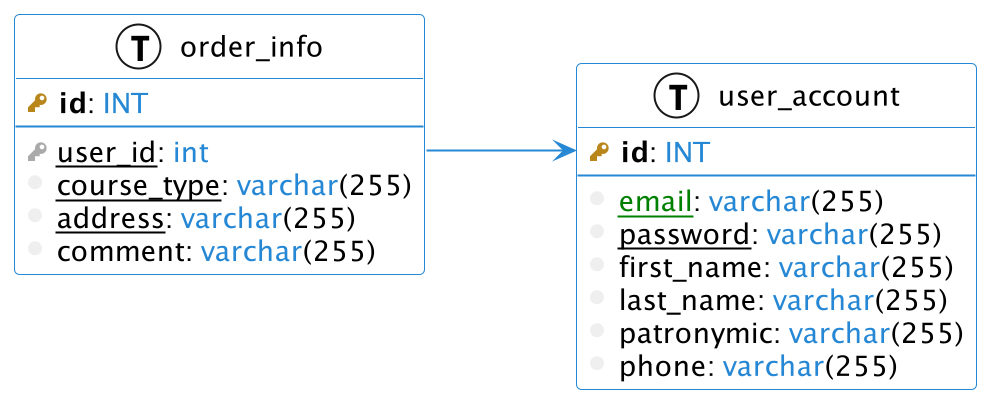
\includegraphics[width=0.7\textwidth]{images/puml/database.png}
  \caption{Схема базы данных}
  \label{fig:puml/database.png}
\end{figure}

\section{Вывод}

В ходе выполнения лабораторной работы я научился создавать веб-страницы с
помощью HTML, CSS и PHP-скриптов, которые взаимодействуют с базой данных MySQL.

\newpage

\appendix

\titleformat{\section}[display]
{\normalfont\bfseries}
{\centering Приложение\ \thesection}
{0pt}{\centering}
\renewcommand{\thesection}{\Asbuk{section}}

\section{Исходный код главной страницы}
\label{app:index.html}

\begin{code}
  \inputminted{html}{../task-1/index.html}
\end{code}

\newpage

\section{Исходный код страницы входа в аккаунт}
\label{app:login.html}

\begin{code}
  \inputminted{html}{../task-1/login.html}
\end{code}

\newpage

\section{Исходный код страницы успешного входа в аккаунт}
\label{app:login-success.html}

\begin{code}
  \inputminted{html}{../task-1/login-success.html}
\end{code}

\newpage

\section{Исходный код страницы оформления заказа}
\label{app:order.html}

\begin{code}
  \inputminted{html}{../task-1/order.html}
\end{code}

\newpage

\section{Исходный код страницы успешного оформления заказа}
\label{app:order-success.html}

\begin{code}
  \inputminted{html}{../task-1/order-success.html}
\end{code}

\newpage

\section{Исходный код стилей}
\label{app:style.css}

\begin{code}
  \inputminted{css}{../task-1/css/style.css}
\end{code}

\newpage

\section{Исходный код скрипта работы с БД}
\label{app:database.php}

\begin{code}
  \inputminted{php}{../task-1/database.php}
\end{code}

\newpage

\section{Исходный код скрипта входа в аккаунт}
\label{app:login.php}

\begin{code}
  \inputminted{php}{../task-1/login.php}
\end{code}

\newpage

\section{Исходный код скрипта оформления заказа}
\label{app:order.php}

\begin{code}
  \inputminted{php}{../task-1/order.php}
\end{code}

\end{document}
